\section{第七章\quad 气体与蒸汽的流动}

% 1,2,3,5,6，也就是 ppt 上的所有内容

\pt{三维非定常流动连续性方程}：$\frac{\partial\rho}{\partial t}+\frac{\partial(\rho u)}{\partial x}+\frac{\partial(\rho v)}{\partial y}+\frac{\partial(\rho w)}{\partial z}=0$;

\pt{连续性方程}：$\frac{Ac_\mathrm{f}}{\nu}=\text{const.}$;

\pt{微分形式}：$\frac{\mathrm{d}\nu}{\nu}=\frac{\mathrm{d}A}{A}+\frac{\mathrm{d}c_\mathrm{f}}{c_\mathrm{f}}$ 或 $\frac{\mathrm{d}\rho}{\rho}+\frac{\mathrm{d}A}{A}+\frac{\mathrm{d}c_f}{c_f}=0$;

\pt{绝热方程}: $pv^\kappa=\mathrm{const.}$ 微分形式：$\kappa\frac{\mathrm{d}v}{v}+\frac{\mathrm{d}p}{p}=0$；注意，水蒸气中的 $\kappa\ne \frac{c_p}{c_V}$；

\pt{稳定流动能量方程}：$q=\Delta h+\frac{1}{2}\Delta c_f^2+g\Delta z+w_s$， 喷管等问题中常取 $q\approx 0$、$w_s=0$，并忽略 $g\Delta z$，于是：$h+\frac{c_f^2}{2}=\mathrm{const.}$，微分形式为 $\mathrm{d}h+c_f\,\mathrm{d}c_f=0$

\pt{绝热滞止状态}：若流体被绝热、可逆地减速到 $c_f\to 0$，则焓达到最大值：$h_0=h_1+\frac{c_{f1}^2}{2}$， $h_0$ 称为总焓或滞⽌焓

\pt{理想气体、定比热时滞止参数}： $T_0=T_1+\frac{c_{f1}^2}{2c_p},p_0=p_1\left(\frac{T_0}{T_1}\right)^{\frac{\kappa}{\kappa-1}},v_0=\frac{R_gT_0}{p_0}$。若为水蒸气则使用前面两个方程再由水蒸气性质图查到

\pt{拉普拉斯声速方程}：$c=\sqrt{\left(\frac{\partial p}{\partial \rho}\right)_s}=\sqrt{-v^2\left(\frac{\partial p}{\partial v}\right)_s}$。等熵过程中 $c=\sqrt{\kappa pv}=\sqrt{\kappa R_\mathrm{g}T}$。\pt{当地声速}是考虑的某留到某一截面上的声速。\pt{马赫数} $\mathrm{Ma}=\frac{c_f}{c}$

\divider

\pt{气体流速改变的力学条件}：$-\frac{\mathrm{d}p}{p}=\kappa \mathrm{Ma}^2\frac{\mathrm{d}c_f}{c_f}$，可以通过流动的能量方程和热力学第一定律的第二解析式得到，速度升高的能量来源是焓㶲转换为机械能。结合绝热过程方程得到 $\mathrm{Ma}^2\frac{\mathrm{d}c_f}{c_f}=\frac{\mathrm{d}v}{v}$

\pt{几何条件}：$\frac{\mathrm{d}A}{A}=\left(\mathrm{Ma}^2-1\right)\frac{\mathrm{d}c_f}{c_f}$。亚音速加速需要渐缩喷管；超音速加速需要渐扩喷管；音速流动时气体截面收缩至最小，此时的\pt{临界截面（喉部截面）}上的 $p_{\mathrm{cr}},T_{\mathrm{cr}},v_{\mathrm{cr}}$ 分别称为临界压力、临界温度、临界比体积。使得气体从亚音速加速到超音速的喷管为\pt{渐缩渐扩喷管}，称为\pt{拉伐尔喷管}

\pt{扩压管}的目的是使得 $p$ 上升，$c_f$ 下降，$\mathrm{Ma}$ 下降，将动能转换为压力势能

\divider

\pt{流速计算}：$c_{f2}=\sqrt{2(h_0-h_2)}=\sqrt{2(h_1-h_2)+c_{f1}^2}$ 适用于绝热、不做功的任意工质。
\pt{理想气体、定比热容}：$c_f=\sqrt{2c_p(T_0-T_2)}=\sqrt{2\frac{\kappa R_{\mathrm{g}}}{\kappa-1}(T_{0}-T_{2})}$，$T_0$ 为滞止温度, $T_0=T_1+\frac{c_{f1}^2}{2c_p},p_0=p_1\left(\frac{T_0}{T_1}\right)^{\frac{\kappa}{\kappa-1}},v_0=\frac{R_gT_0}{p_0}$ \\
若可逆 $c_f=\sqrt{\frac{2\kappa}{\kappa-1}R_gT_0\left[1-\left(\frac{p_2}{p_0}\right)^{\frac{\kappa-1}{\kappa}}\right]}$

\pt{临界压力比}：$\nu_{\mathrm{cr}}=\frac{p_{\mathrm{cr}}}{p_0}=\left(\frac{2}{\kappa+1}\right)^{\frac{\kappa}{\kappa-1}}$

\pt{背压对流速的影响}

\begin{itemize}
    \item \pt{收缩喷管}：若 $p_b>p_{\mathrm{cr}}$，则 $p_2=p_b$，$c_{f2}<c_2$，$\mathrm{Ma}_2<1$。
    \item \pt{收缩喷管}：若 $p_b\le p_{\mathrm{cr}}$，则 $p_2=p_{\mathrm{cr}}$，$c_{f2}=c_2$，$\mathrm{Ma}_2=1$，发生临界流动。
    \item \pt{缩放喷管}：只讨论 $p_b<p_{\mathrm{cr}}$ 的情况，此时 $p_{\mathrm{thr}}=p_{\mathrm{cr}}$，$c_{f,\mathrm{thr}}=c_{\mathrm{cr}}$，$\mathrm{Ma}_{\mathrm{thr}}=1$，出口可达 $\mathrm{Ma}_2>1$。
\end{itemize}

\pt{流量计算}：$q_m=\frac{A c_f}{v}=\rho A c_f$， 通常收缩喷管按出口截面计算；缩放喷管可按喉部截面或出口截面计算。理想气体、定比热容、绝热时 $q_m=A_2\sqrt{\frac{2\kappa}{\kappa-1}\frac{p_0}{v_0}\left[\left(\frac{p_2}{p_0}\right)^{\frac{2}{\kappa}}-\left(\frac{p_2}{p_0}\right)^{\frac{\kappa+1}{\kappa}}\right]}$

\begin{itemize}
    \item 当 $\frac{p_2}{p_0}=1$ 时，$q_m=0$，$c_{f2}=0$。
    \item 当 $\nu_{\mathrm{cr}}<\frac{p_2}{p_0}<1$ 时，$\frac{p_2}{p_0}\downarrow$，$c_{f2}\uparrow$，$q_m\uparrow$。
    \item 当 $\frac{p_2}{p_0}=\nu_{\mathrm{cr}}$ 时，$p_2=p_{\mathrm{cr}}$，$c_{f2}=c_2$，$q_m=q_{m,\max}$。
    \item 当 $\frac{p_2}{p_0}<\nu_{\mathrm{cr}}$ 时，收缩喷管已堵塞，流量仍为 $q_{m,\max}$。
\end{itemize}

\noindent
\begin{minipage}
    [t]{0.48\linewidth}
    \vspace{0pt}
    \raggedright
    \pt{喷管设计任务}：已知 $p_1$,$v_1$,$T_1$,$c_{f1}$,$p_b$,$P$ 确定喷管形状和几何尺寸。\\
    \pt{外形选择}：先比较 $p_{\mathrm{cr}}$ 与 $p_b$，再决定收缩喷管或缩放喷管。\\
    \pt{几何尺寸}：$A_2=\frac{q_m v_2}{c_{f2}}$，$A_{\mathrm{thr}}=\frac{q_m v_{\mathrm{cr}}}{c_{f,\mathrm{cr}}}$，$l=\frac{d_2-d_{\min}}{2\tan(\varphi/2)}$
\end{minipage}
\hfill
\begin{minipage}
    [t]{0.48\linewidth}
    \vspace{0pt}
    \centering
    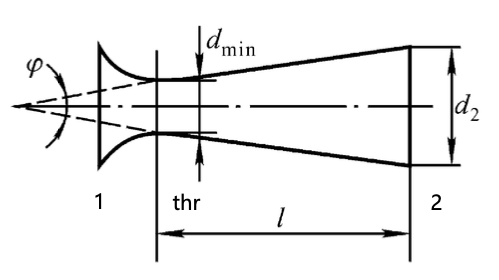
\includegraphics[width=\linewidth]{figures/7喷管设计.png}
\end{minipage}

\divider

摩擦使实际出口速度小于可逆绝热出口速度 $c_{f2}<c_{f2s}$。\\
\pt{喷管速度系数} $\varphi=\frac{c_{f2}}{c_{f2s}}$，一般取 $0.92\sim 0.98$。\\
\pt{能量损失系数}：$\zeta=\frac{c_{f2s}^2-c_{f2}^2}{c_{f2s}^2}=1-\varphi^2$，\\
\pt{喷管效率}：$\eta_N=\frac{c_{f2}^2}{c_{f2s}^2}=\frac{h_0-h_2}{h_0-h_{2s}}=\varphi^2$，$\zeta=1-\eta_N$\\
\pt{摩擦引起的作功能力损失}：$I=\frac{1}{2}\left(c_{f2s}^2-c_{f2}^2\right)$

\divider

\noindent
\begin{minipage}
    [t]{0.48\linewidth}
    \vspace{0pt}
    绝热节流前后焓几乎不变，但是非等焓过程，\\强烈不可逆 $s_2>s_1$，\\做工能力损失 $I=T_0s_g=s_2-s_1$\\
    焦耳-汤姆逊系数：$\mu_J=\left(\frac{\partial T}{\partial p}\right)_h=\frac{T\left(\frac{\partial v}{\partial T}\right)_p-v}{c_p}$
\end{minipage}
\hfill
\begin{minipage}
    [t]{0.48\linewidth}
    \vspace{0pt}
    \centering
    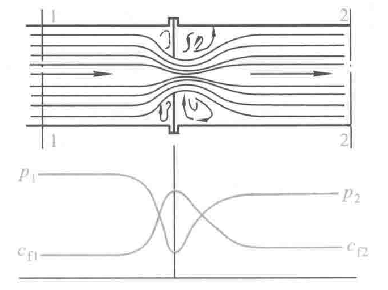
\includegraphics[width=\linewidth]{figures/7绝热节流.png}
\end{minipage}

\begin{itemize}
    \item 若 $T\left(\frac{\partial v}{\partial T}\right)_p-v>0$ 则 $\mu_J>0$，$\mathrm{d}T<0$，节流降温。
    \item 若 $T\left(\frac{\partial v}{\partial T}\right)_p-v<0$ 则 $\mu_J<0$，$\mathrm{d}T>0$，节流升温。
    \item 若 $T\left(\frac{\partial v}{\partial T}\right)_p-v=0$ 则 $\mu_J=0$，$\mathrm{d}T=0$。
\end{itemize}

\pt{回转温度}：节流前后温度保持不变的温度。将气体状态方程带入 $\mu_j$ 式能够得到不同压力下的回转温度，连接得到曲线，根据曲线内外带入点计算 $\mu_J$ 的符号能够判断该点是节流升温还是节流降温。

若为\pt{水蒸气}，则节流后温度稍有下降，前后可取 $h_1=h_1'$，若膨胀到相同压力，节流后的作功能力减少 $(h_1-h_2)-(h_1'-h_2')=h_2'-h_2$，作功能力损失 $I=h_2'-h_2=T_0s_g=T_0(s_1'-s_1)$

\divider